\documentclass[5 pt]{article}
\usepackage{graphics}
\usepackage{graphicx}
\usepackage{geometry}
\usepackage{multicol}
\usepackage{hyperref}
\usepackage{subcaption}
\usepackage{fontawesome5}
%\usepackage{m}
%\usepackage{lipsum}
%\usepackage{mwe}
\usepackage{amsmath}
\geometry{a4paper,left=25mm,right=25mm, top=25mm, bottom=25mm}
\usepackage[none]{hyphenat}
\usepackage{fancyhdr}
\pagestyle{fancy}
\fancyhead{}
\fancyhead[R]{AI in Medicine (Phase II)}
\fancyhead[L]{ML Final Project}
\begin{document}
\begin{titlepage}
\begin{figure}[ht] 

\includegraphics[width=3.5cm]{1.png}


\end{figure}
%()(from right smaller goes left , up and down bigger goes up)
\begin{picture}(50, 135)(-360, -160)
 
\includegraphics[scale=0.5]{2.png}
\end{picture}

\begin{center}

\line(1,0){500}\\
\large \textbf{Artificial Intelligence in Medicine - Final Project(Phase II)\\ }

\vspace{1cm}
\large \textbf{ 10-Year Risk of Death of Individuals from the NHANES I Epidemiology
Dataset}\\
\line(1,0){500} \\
\vspace{2cm}
\faUsers\ Submitted to:\\
Dr. Inas Yassin\\
Eng. Christeen Adly

\vspace{2cm}
\faUser\ Submitted by:\\
\vspace{.5cm}
\begin{tabular}{ ||p{7cm}|p{3cm}|p{3cm}||  }
\hline 
\hline
Name & Sec & BN \\
\hline
Mohamed Ahmed Abdelaziz & 2 & 14 \\ 
\hline 
 Mohamed Khaled Galloul& 2 & 15 \\ 
\hline 
Mohamed Abdelkareem Seyam & 2 & 18 \\ 
\hline 
Ahmed Mohamed Mohamed & 1 & 7 \\
\hline 
\hline
\end{tabular}


\vspace{1cm}
 Cairo University\\
Please let us know if we need to provide any further details.\\
\underline{\faEnvelope\ \href{mailto:mohamed.ahmed997@eng-st.cu.edu.eg}{mohamed.ahmed997@eng-st.cu.edu.eg}}\\
\underline{\faEnvelope\ \href{mailto:mohamed.attia99@eng-st.cu.edu.eg}{mohamed.attia99@eng-st.cu.edu.eg}}


\end{center}
\end{titlepage}


\tableofcontents
\vspace{8cm}
\listoffigures
\newpage


\section{Preprocessing}

\textbf{\underline{\href{https://github.com/mohamed-abdelaziz721/ml-final-project/blob/main/PhaseI.pdf}{Please refer to phase I for data description [click this line to be redirected to the pdf]}}}

\subsection{Handling Missing Data}
After Examining the data we find that "Systolic BP" feature has more than 50\% of missing values. We will describe different approaches to deal with this problem in section 2.2.
\subsection{Balancing the Data}
We will use up-sampling using 'SMOTE' which stands for Synthetic Minority Over-Sampling Technique. SMOTE is performing the same basic task as basic re-sampling (creating new data points for the minority class) but instead of simply duplicating observations, it creates new observations along the lines of a randomly chosen point and its nearest neighbors.
\begin{itemize}
    \item \textbf{Before up-sampling:} number of true predictions [6954], number of false predictions [1625].  
    \item \textbf{After up-sampling:} number of true predictions [6954], number of false predictions [6954].
\end{itemize}


\subsection{Scaling/Normalizing the Data}
We can apply the StandardScaler to our dataset directly to standardize the input variables. We will use the default configuration and scale values to subtract the mean to center them on 0.0 and divide by the standard deviation to give the standard deviation of 1.0. 


\section{Evaluation Metric}
\subsection{Concordance index (C-index)}
The concordance index (c-index): is a metric to evaluate the predictions made by an algorithm. It is defined as the proportion of concordant pairs divided by the total number of possible evaluation pairs.
$$ \textrm{c-index}= \frac{\textrm{the proportion of concordant pairs } + 0.5  \textrm{ x number of ties}}{\textrm{total number of possible evaluation pairs}} $$
\begin{itemize}
\item the concordance index is interested on the order of the predictions, not the predictions themselves. 

\item This is very different from other evaluation measures such as mean squared error or mean absolute error.

\end{itemize}

\textbf{c-index characteristics}\\
\begin{itemize}
    \item  A function of how well the ordered values of the continuous predictor correlate to the corresponding event status.
\item  For an increasing events status any strictly increasing predictions the concordance index will still be equal to 1.
\item The concordance index will be zero for every strictly decreasing predictions.
\item In case of Ties in your predictions they are counted as half concordant pairs.
\item  The concordance index supports right censoring which means that the event of interest has only occurred for a subset of the observations (e.g., `death of a patient`,  `customer unsubscribe` or  `any time to event model`). 

\item Random predictions give a mean concordance index of approximately 0.5. So basically a model that hasn’t learned anything give a mean concordance index of 0.5.
\end{itemize}

\subsection{Effect of Preprocessing on c-index with different approaches}

\subsubsection{data with missing rows dropped ( \(>\)50\% of rows)}
We see that our train and validation sets have missing values, but our test set has no missing values.

we will begin with a  complete case analysis dropping all of the rows with any missing data. Run the following cell to drop these rows from our train and validation sets.

\subsubsection{data after dropping the systolic BP column \& Balancing with Up-Sampling.}
The two methods above show two Decision Tree models \underline{one: with features after balancing and dropping Systolic BP} and \underline{second: with missing rows dropped ( \(>\)50\% of rows dropped)}.

The models predicts that the missing rows drop approach achieved c-index score (\(\approx\) 0.5), but balanced data achieved c-index score (\(\approx\) 0.7) and from that we can deduce two things:
\begin{itemize}
    \item c-index is indeed a very good evaluation metric for `the time to an event models`, as it show the true model performance which in our simple decision tree classifier is random (model learned nothing). c-index is used as the outcome of interest isn't only whether or not an event occurred, but also when that event occurred. 
    \item Tree seems to be overfitting for the first model: it fits the training data so well that it doesn't generalize to other samples such as the validation set.
\end{itemize}


We may now proceed with the balancing approach and dropping the 'Systolic BP' feature, but to make sure we may try mean imputation approach to see how our model would generalize with avoiding complete case analysis.

Later We will also try different classifiers and use Grid Search for Hyper-parameter selection for our best 3 classifiers to improve the c-index score. See Candidate Classification Section


\subsubsection{data after imputation (mean imputation)}

We will try to improve the test C-Index by filling the missing values and explore if the data is missing at random or not (as we threw away more than half of the data for systolic BP instead of imputing).

We will plot histograms of the dropped rows against each of the features and compare these to the histograms of the feature in the entire dataset. Try to see if one of the features has a significantly different distribution in the two subsets.

 \begin{figure}[h]
	\begin{subfigure}{0.5\textwidth}
		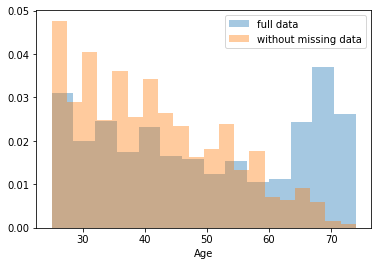
\includegraphics[width=1\linewidth, height=3.5cm]{age.png} 
		\caption{Age Histograms}
	\end{subfigure}
	\begin{subfigure}{0.5\textwidth}
		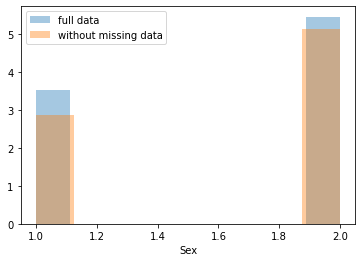
\includegraphics[width=1\linewidth, height=3.5cm]{sex.png}
		\caption{Sex Histograms}
	\end{subfigure}
	\begin{subfigure}{0.5\textwidth}
		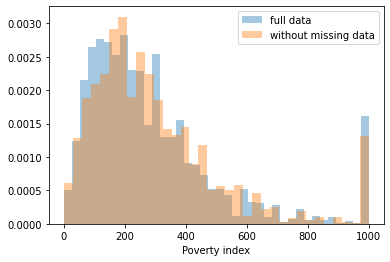
\includegraphics[width=1\linewidth, height=3.5cm]{pov.png}
		\caption{Poverty Index Histograms}
	\end{subfigure}
\caption{histograms of the dropped rows against some of the features compared to the histograms of the features in the entire dataset}
\label{fig:image2}
\end{figure}

\newpage
Most of the features are distributed similarly whether or not we have discarded rows with missing data. In other words missingness of the data is independent of these features.

If similar distribution was true across all features, then the data would have been said to be missing completely at random (MCAR).\\
But when considering the age feature, we see that much more data tends to be missing for patients over 65. The reason could be that blood pressure was measured less frequently for old people to avoid placing additional burden on them.\\
As missing values is related to one or more features, the missing data is said to be missing at random (MAR) and we will replace the missing values with mean substitution approach



\textbf{
\begin{itemize}
    \item We should see that avoiding complete case analysis (dropping rows with missing values) allows our model to generalize a bit better.
\item We Will now proceed with the balanced data and with the systolic BP dropped as it had the best score
\end{itemize}
}

\section{Candidate Features}

\subsection{Permutation Importance}
\begin{itemize}
    \item Feature importance applied after the model has been fitted.
    \item It selects each feature column one at a time and shuffles/permutate that column randomly. Then it calculates how that affect the prediction/accuracy of the model
    \item If changing value of a feature column affect the accuracy of the model heavily then the importance of that column feature is higher. In this way, feature importance is calculated.\\
    
    \begin{figure}[h]
	\centering
	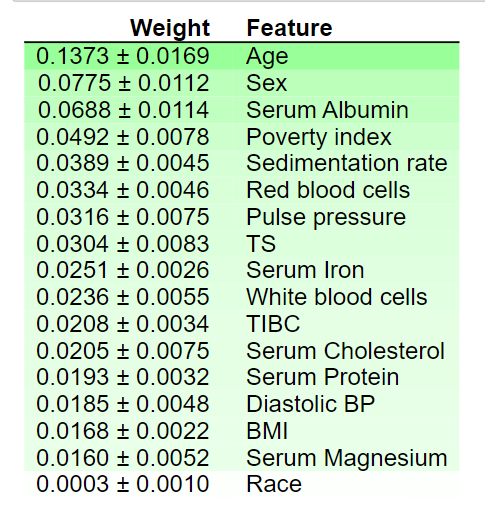
\includegraphics[width=.5\textwidth, height =.28\textheight]{fs.png}
	\caption{Features importance ranked by permutation importance}
	\end{figure}

\end{itemize}

\textbf{Now we know a lot of inside in our model by using feature importance. We can use this information when collecting dataset and pay more attention to the important features and may discard the features that lower the model performance.}\\


\textbf{\underline{Note:even after removing 5 features (least permutation score) the testing c-index doesn't change as much from our best preprocessing technique on all the features.}}


\subsection{PCA (Dimentionality reduction)}
After performing the PCA we can notice that even when choosing high number of principal components the model performance wasn't better than removing  the least relevant features from the permutation\\

Now we will fed our models with the data which was calculated using:
\begin{itemize}
    \item Data after dropping the systolic BP ( \(>\) 50\% missing) \& Balancing with Up-Sampling.
    \item Feature Selection using permutation importance
\end{itemize}




\section{How a single feature affect our prediction (PDP)}
we previously had the most important features of our model. It's a good insight, but we don't know how each feature affecting accuracy (Is sex increasing or decreasing the risk of death?).

Partial Dependance Plot (PDP): shows how each feature will affect the prediction of the model increase or decrease
\begin{itemize}
    \item PDP calculated after a model is fitted.
    \item Use single row for prediction. Repeatedly alter a variable value to make a series prediction.
    \item  Do that for multiple rows and plot the average prediction on the vertical axes
\end{itemize}


\begin{figure}[h]
	\begin{subfigure}{0.5\textwidth}
		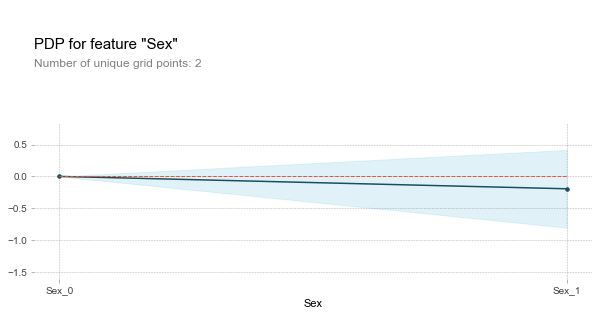
\includegraphics[width=1\linewidth, height=3.5cm]{pdpsex.png} 
		\caption{Sex}
	\end{subfigure}
	\begin{subfigure}{0.5\textwidth}
		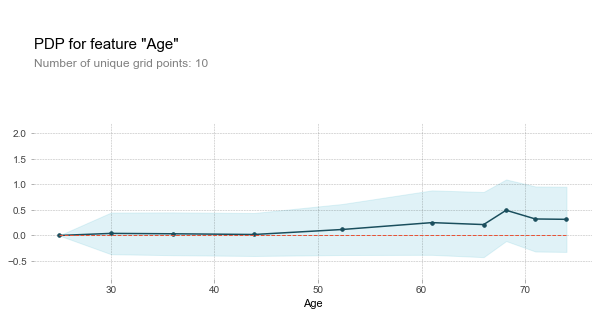
\includegraphics[width=1\linewidth, height=3.5cm]{pdpage.png}
		\caption{Age}
	\end{subfigure}
	\begin{subfigure}{0.5\textwidth}
		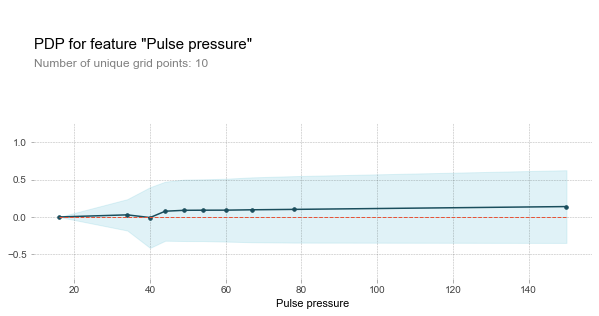
\includegraphics[width=1\linewidth, height=3.5cm]{pdppp.png}
		\caption{Pulse Pressure}
	\end{subfigure}
	\begin{subfigure}{0.5\textwidth}
		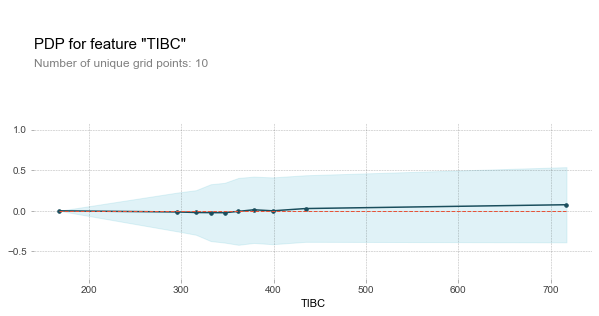
\includegraphics[width=1\linewidth, height=3.5cm]{pdptibc.png}
		\caption{TIBC}
	\end{subfigure}
	
\caption{Partial Dependence Plots:The y axis is interpreted as change in the prediction from what it would be predicted at the baseline or leftmost value. A blue shaded area indicates level of confidence (standard deviation). }
\label{fig:image2}
\end{figure}

\begin{itemize}
    \item \textbf{PDP(Sex)} The probability of death risk is decreased in females [ poor men! :( ].
    \item \textbf{PDP(Age)} The probability of death risk is decreased if the age is over 60
    \item \textbf{PDP(Pulse pressure)} In the third plot, we see that death risk probability increases after pulse pressure hits 80.
    \item \textbf{PDP(TIBC)} Lastly, we see that death risk probability increases,but not significant, after TIBC hits 410.
\end{itemize}



\section{Why my model predicted that (SHAP Values)}

In the previous section, we already have seen how our model works, which features are important and how individuals feature affect the prediction of our model. But now we want to know why an individual prediction is made. Why our model made such a prediction?

SHAP Values (an acronym from SHapley Additive exPlanations) break down a prediction to show the impact of each feature. It explains why a model made a certain prediction. Previously, we see the explanation of the model after training and how each feature will affect the prediction of the model. Now we are going to look at the individual prediction that our model made. Meaning we will now look at our model after it has made a prediction.



How much a prediction is driven by the factor of sex or pulse presure instead of some baseline value of them? And we do these for each feature. The rules for calculating SHAP values is:

$$\textrm{sum(SHAP values for all features) = pred for patient - pred for baseline values}
$$

\begin{itemize}
    \item SHAP: how each feature affected the prediction (after prediction).
\item It calculates how the value of a feature affected the predicted outcome instead of some baseline value.
\item It does it for every feature and shows the contribution of each feature for the outcome.
\item SHAP interpret how feature increase or decrease prediction with reference to the PDP and show how consistent your results
\end{itemize}

    \begin{figure}[h]
	\centering
	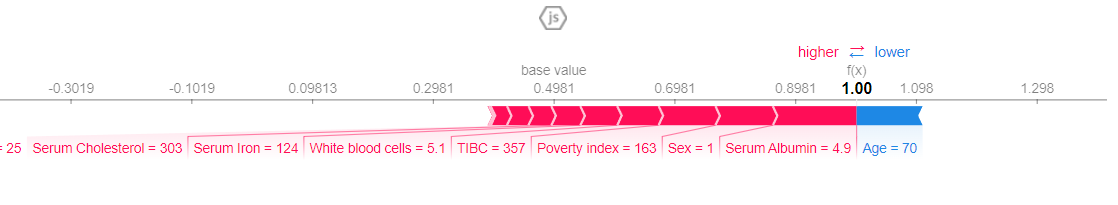
\includegraphics[width=1\textwidth, height =.15\textheight]{shap.png}
	\caption{SHAP for a true prediction}
	\end{figure}

    \begin{figure}[h]
	\centering
	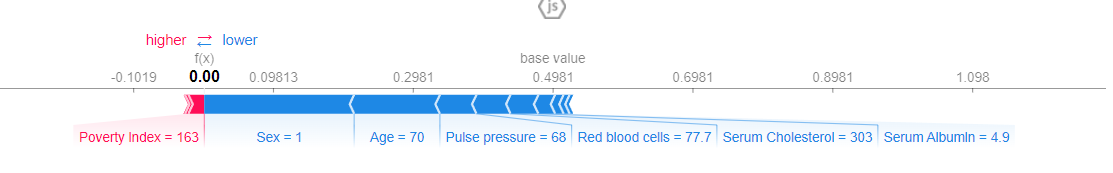
\includegraphics[width=1\textwidth, height =.15\textheight]{shap2.png}
	\caption{SHAP for a true prediction}
	\end{figure}

From the two shap plots ubove we can see that the most important features we get from permutation importance are the most relevant in the prediction and with shap we can see each feature contribution either it increase or decrease the prediction.


\section{Candidate Classification Techniques}
We Started fitting numerous models [LogisticRegression, KNN, SVM, DecisionTree, RandomForest, XGBoost, NaiveBayes, HistGradientBoosting] to \textbf{choose the best 3 base classifiers} to use in our \textbf{ensemble voting technique} after performing \textbf{hyper-parameter grid search} on them. 


The Best 3 models based on c-index testing score was 
\begin{itemize}
    \item RandomForest: 0.865
    \item XGBoost: 0.879
    \item HistGradientBoost: 0.865
\end{itemize}

\subsection{Grid Search and voting classifier}
This function helps to loop through predefined hyper-parameters and fit your estimator (model) on your training set.\\

The grid search of each classifier uses the following hyper-parameters:

\begin{itemize}
    \item RandomForest: [n-estimators, max-depth, max-features] \(\longrightarrow\) 0.863
    \item XGBoost: [n-estimators, eta, gamma, max-depth, subsample, colsample-bytree]  \(\longrightarrow\) 0.887
    \item HistGradientBoost: [max-iter, learning-rate, max-depth, max-leaf-nodes]  \(\longrightarrow\) 0.869
\end{itemize}

\textbf{Voting Classifier} \(\longrightarrow\) 0.883



 

\end{document}




